\documentclass[12pt]{article}

\usepackage{physics} % provides lots of nice features and commands often used in physics, it also loads some other packages (like AMSmath)
\usepackage{siunitx} % typesets numbers with units very nicely
\usepackage{enumerate} % allows us to customize our lists

\begin{document}

\title{Joke Generator}
\author{Timur Aizatvafin, Vsevolod Mikulik, Andrey Starodumov}

\maketitle

\begin{abstract}
	This report describes our attempts at joke generation. Briefly speaking, we tried both fine-tuning a pre-trained GPT-2 and
    training a GPT from scratch (with resources available, of course).
\end{abstract}

\section{Fine-tuning a pre-trained GPT2}
As the pre-trained model, we used GPT2LMHeadModel model from an OpenAI adn trained it on the \href{https://www.kaggle.com/datasets/abhinavmoudgil95/short-jokes}{shortjokes dataset}.
    
\subsection{Data Preprocessing}
Each joke was tokenized by the GPT2Tokenizer with its embedded vocab.

\subsection{Training}
For the training process we used the model function that allows to put the input data and desired output data in the model. After this the model calculates its loss by shifting the desired output data and comparing with model prediction. So the model calculates if it predicted next words correctly.

[Figure \ref{pic:gpt2-loss}] shows how loss was decreasing during the training.

\begin{figure*}[ht]
\caption{Losses of pre-trained model}
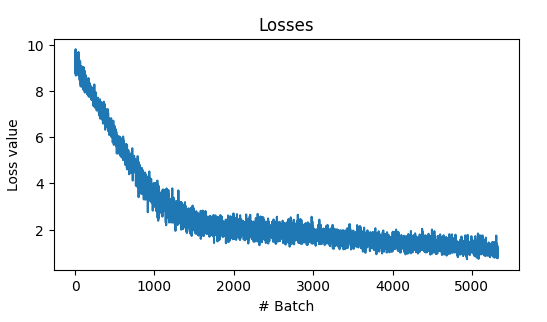
\includegraphics[width=\textwidth]{gpt2-loss.png}
\label{pic:gpt2-loss}
\end{figure*}

\subsection{Results}
The result is not impressive, but sometimes the model makes funny jokes.
Here you can see the few generated jokes:
\begin{itemize}
    \item Input: \textit{"The president kills"} \\
    Output: \textit{"The president kills the people who make the best decisions"}
    \item Input: \textit{"What is your"} \\
    Output: \textit{"What is your greatest weakness? Your inability to read the words on your resume"}
    \item Input: \textit{"Who is"} \\
    Output: \textit{"Who is the most popular person in the world? The one who can count"}
\end{itemize}

\section{Training a GPT from Scratch}

We also came up with an idea of training a GPT from scratch. We found an implementation [TODO: parameters] and trained it on the dataset
of jokes from Reddit [TODO: link].

\subsection{Data Preprocessing}

\paragraph{}
Dataset of our choice is a simple .csv file with each entry being a complete joke.

[image here]

\paragraph{}
In order to train the model, we decided to
\begin{enumerate}
	\item Tokenize each entry
	\item Add "end of text" token to each entry
	\item Combine all preprocessed entries into a single long list of tokens
\end{enumerate}

\subsection{Training}



\subsection{Results}

\section{Conclusion}



\end{document}